%%%%%%%%%%%%%%%%%%%%%%%%%%%%%%%%%%%%%%%%%%%%%%%%%%%%%%%%%%%%%

\mainmatter
\setcounter{page}{1}

\lectureseries[\course]{\course}

\auth[\lecAuth]{Lecturer: \lecAuth\\ Scribe: \scribe}
\date{January 19, 2010}

\setaddress

% the following hack starts the lecture numbering at 1
\setcounter{lecture}{4}
\setcounter{chapter}{4}

\lecture{Fundamental Properties of Nonlinear Systems II}

\section{Continuity}
This lecture is focused on continuity as found in Chapter 3 of Khalil.

\begin{theorem}
\label{th:05lip}
Consider $\dot{x} = f(t,x)$. Let $f(t,x)$ be piecewise continuous in $t$ and Lipschitz in $x$ such that
$$|f(t,x) - f(t,y)| \leq L|x-y|, ~\forall x,y\in\mathcal{B} = \{x\in\mathbb{R}^n ~|~ |x-x_0|\leq r\}, ~\forall t\in[t_0,t_1]$$
where $L>0$ is a constant. Then there exists $\delta>0$ such that the system has a unqiue solution over $[t_0,t_0+\delta]$ with $t_0+\delta\leq t_1$.
\end{theorem}

The important condition is the Lipschitz inequality. Note that
$$\mathcal{C}^0 \Leftarrow \text{Lipshcitz} \Leftarrow \mathcal{C}^1$$
where $\mathcal{C}^0$ means a function is continuous and $\mathcal{C}^1$ means a function is differentiable and smooth. This theorem is really saying that for some finite, positive amount of time, $t_0+\delta$, the system will not blow up. Also, note that $\delta\sim\frac{1}{L}$.

The piecewise continuous condition only needs to be satisfied such that there is more than an infinitesimal amount of time between switching, for example in a system with relays. This theorem holds for $\delta$ amount of time where $\delta$ is based on the initial conditions $x_0$.

\begin{example}
Figure \ref{fig:05lip} shows two examples of functions where $L=1$. They are both Lipschitz, and therefore $\mathcal{C}^0$, but not $\mathcal{C}^1$. To see that $L=1$ take any two points, find the slope (in absolute value terms) and that slope will always be less than or equal to one.
$\lozenge$
\end{example}

\begin{figure}[ht!]
	\centering
	\includegraphics[width=.7\textwidth]{images/05lip}
	\caption{Two functions that are Lipschitz with $L=1$.}
	\label{fig:05lip}
\end{figure}

\begin{example}
Figure \ref{fig:05notlip} shows a function that is $\mathcal{C}^0$ but not Lipschitz. Near the origin the slope is infinite. Note that if we consider only the range $[0+\epsilon,\infty)$ then this function is Lipschitz and $\mathcal{C}^1$.
$\lozenge$
\end{example}

\begin{figure}[ht!]
	\centering
	\includegraphics[width=.5\textwidth]{images/05notlip}
	\caption{The function $f(x) = \sqrt{x}$ is not Lipschitz.}
	\label{fig:05notlip}
\end{figure}

\begin{definition}
The \textit{Euclidean norm} of a matrix is given as
$$|P| = \sqrt{\lambda_{\text{max}}(P^TP)}$$
\end{definition}

\begin{lemma}
If
$$\left|\frac{\partial f}{\partial x}(t,x)\right| \leq L$$
it follows that the function $f$ is Lipschitz with $L$.
\end{lemma}
For terminology we can interchange Lipschitz, Lipschitz continuous and locally Lipschitz.

\begin{definition}
A function is \textit{globally Lipschitz} if there exists a single $L$ for all $x,y\in\mathbb{R}^n$.
\end{definition}

\begin{example}
The function $f(x) = x^2$ is locally but not globally Lipschitz because $L\to\infty$ as $x\to\infty$. Also, note that $\frac{\partial f}{\partial x} = 2x$ is not bounded. This is a necessary but not sufficient property to show that a function is not Lipschitz.
$\lozenge$
\end{example}

\section{Globally Lipschitz Functions}
All linear, time varying (or time invariant) systems, even unstable ones, are globally Lipschitz.

\begin{example}
This is Example 3.4 in Khalil. Consider
$$\dot{x} = (1+t^2\sin(t))x + t^3\cos(t)$$
The right hand side is globally Lipschitz and $L$ grows with time.
$\lozenge$
\end{example}

If there is strong (quadratic) damping then we fail Lipschitz but we know that there are systems with damping that do not blow up. We will try to clear up this inconsitency later.

\begin{example}
This is Example 3.5 in Khalil. Consider
$$\dot{x} = -x^3 \Rightarrow x(t) = \frac{x_0}{\sqrt{1+2x_0^2t}}$$
This function is locally but not globally Lipschitz.
$\lozenge$
\end{example}

\section{Continuation of Solutions}
Theorem \ref{th:05lip} can be applied repeatedly to get
\begin{align*}
\left[\begin{array}{c} t_0 \\ x(t_0) \end{array}\right] \xrightarrow{\delta}
\left[\begin{array}{c} t_0+\delta \\ x(t_0+\delta) \end{array}\right] \xrightarrow{\delta_2}
\left[\begin{array}{c} t_0+\delta+\delta_2 \\ x(t_0+\delta+\delta_2) \end{array}\right] \rightarrow
\cdots \rightarrow
\left[\begin{array}{c} T \\ x(T) \end{array}\right]
\end{align*}
The range $[t_0, T]$ gives the maximal interval of existence for the solution of a system. In the above expression the $\delta$ intervals will likely get smaller and smaller at each step and converge at a finite time $T$. However, $x(T)$ may be infinite or non-unique. Note that this concept is just a theoretical construct to show that the Theorem \ref{th:05lip} is to be applied multiple times.

\begin{example}
Consider
$$\dot{x} = x^3 \Rightarrow x(t) = \frac{x_0}{\sqrt{1-2x_0^2t}}$$
The maximal interval of existence is $t=[0,\frac{1}{2x_0^2})$.
$\lozenge$
\end{example}

\begin{theorem}
If a function $f$ is globally Lipschitz in $x$ then $\dot{x}=f(t,x)$ has a unique solution for all time.
\end{theorem}

Theorem \ref{th:05lipbound} is a crucial theorem to understand for the remainder of this course.
\begin{theorem}
\label{th:05lipbound}
Let the function $f$ be Lipschitz. Suppose it is also known that every solution of $\dot{x}=f(t,x)$ is bounded. Then there is a unique solution defined for all $t\geq t_0$.
\end{theorem}

The crucial part involves some energy analysis to show that the solution $x(t)$ is bounded. This is what the rest of this course will be studying.

\section{Sensitivity Equations}
This corresponds to Chapter 3.3 of Khalil. We now want to look at systems where
$$\dot{x} = f(t,x,\lambda)$$
By sensitivity we mean the derivative. We are interested in how uncertainties or changes in a system's properties (such as mass, length, etc.) will affect the system behavior.
%%%%%%%%%%%%%%%%%%%%%%%%%%%%%%%%%%%%%%%%%%%%%%%%%%%%%%%%%%%%%